\sect{Metodología de trabajo}{metodologia}

Para el desarrollo de la aplicación se ha utilizado el marco de trabajo \boldFont{SCRUM}, que se emplea para la gestión
de proyectos ágiles de manera \boldFont{iterativa} e \boldFont{incremental}.\ Iterativa porque se revisa y mejora
el producto existente en cada ciclo de desarrollo (\boldFont{sprint}), e incremental porque las nuevas
funcionalidades se integran en la aplicación a medida que se completan.\ Todas las funcionalidades a implementar se
denominan \boldFont{historias de usuario} y forman lo que se denomina Pila del Producto (\boldFont{Product Backlog}).
En cada iteración se seleccionan las historias de usuario que se consideran más prioritarias y se asignan a los
miembros del equipo de trabajo, formando la Pila del Sprint (\boldFont{Sprint Backlog}).

La duración de las iteraciones en SCRUM es variable, pero se recomienda que no sea inferior a 2 semanas.\ En este
proyecto se ha optado por una duración de 4 semanas, ya que el tiempo de desarrollo de cada iteración debe ser
suficiente para que el desarrollador pueda completar todas las tareas que se le han asignado durante la misma.

Puesto que el equipo de trabajo está formado por un único miembro, no ha sido necesario realizar reuniones de
coordinación, porque se ha podido trabajar de manera autónoma y sin necesidad de supervisión.\ Además, se ha
adaptado el marco de trabajo para que se ajuste a las necesidades del proyecto.

La gestión de la pila del producto se ha realizado con la herramienta \boldFont{Notion}, que permite crear espacios
de trabajo con diferentes vistas para organizar las tareas.\ En la figura~\ref{fig:notion-product-backlog} se presenta
una pequeña muestra de la pila del producto.\ Para una descripción más detallada y completa de las tareas realizadas
durante el desarrollo del proyecto, se puede consultar el anexo~\ref{anx:product-backlog-notion}.

\begin{figure}[H]
	\centering
	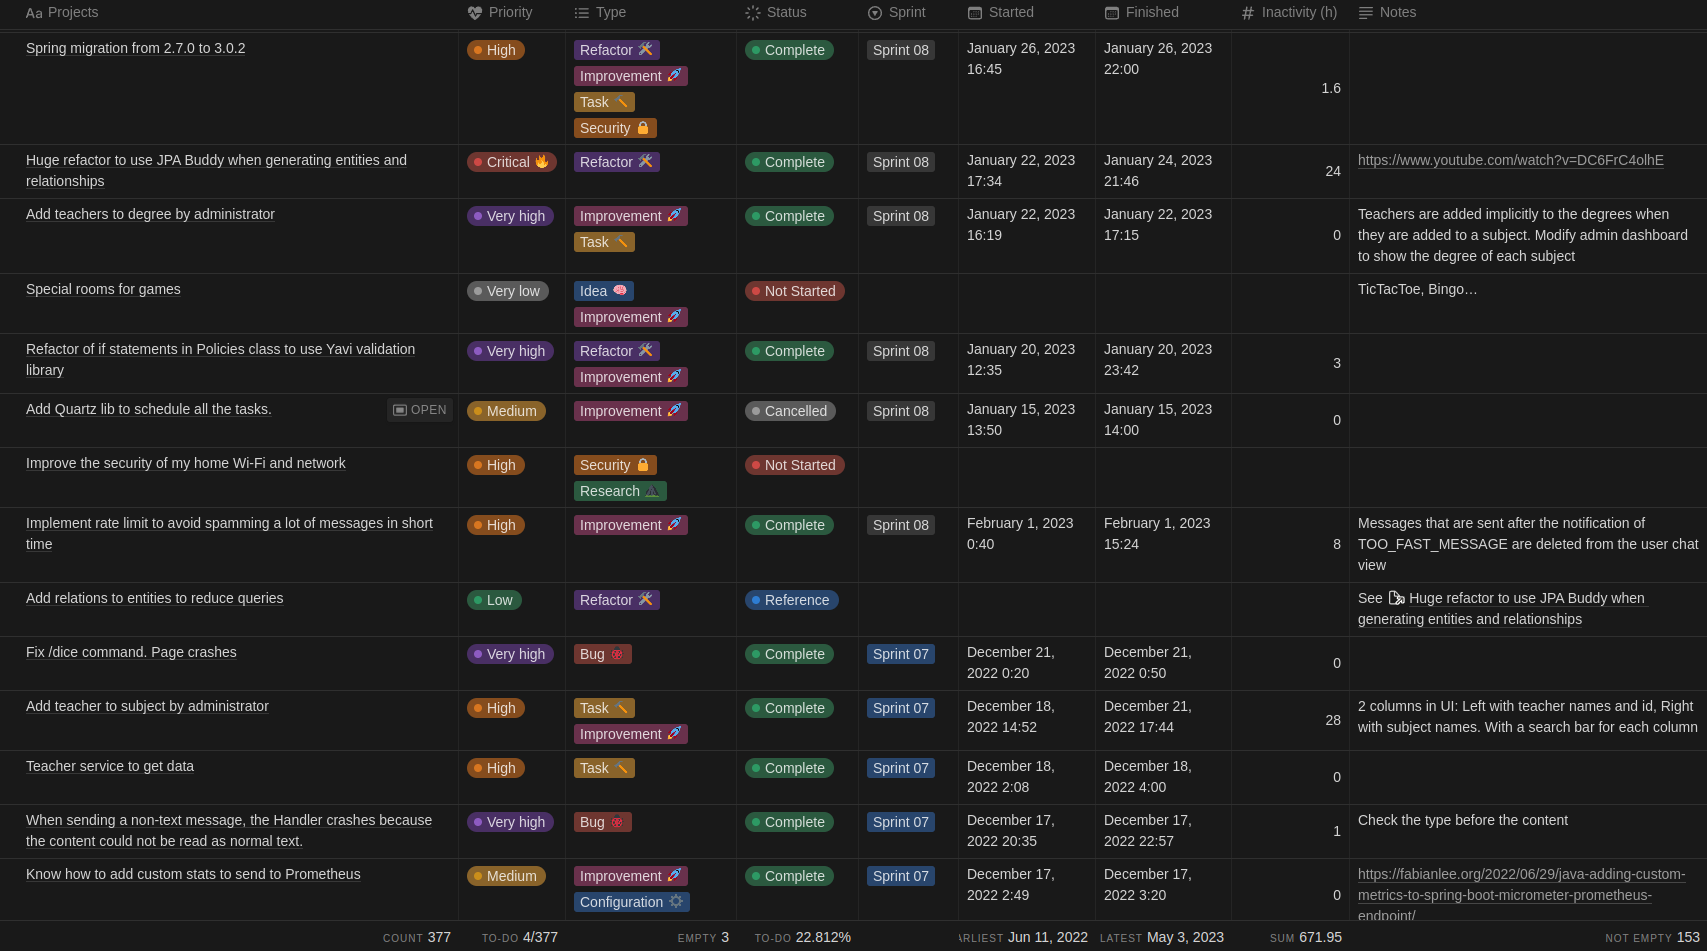
\includegraphics[width=\textwidth]{notion-product-backlog}
	\caption{Pila del producto en Notion}
	\label{fig:notion-product-backlog}
\end{figure}

\sect{Sprints de desarrollo}{sprints-desarrollo}
\subsect{Sprint 1}{sprint1}

Objetivo:

Fecha de inicio: 11/06/2022

Fecha de fin: 11/07/2022

Descripción:

\subsect{Sprint 2}{sprint2}

\underline{Fecha de inicio}: 11/07/2022

\underline{Fecha de fin}: 11/08/2022

\underline{Objetivos}:
\begin{itemize}
	\item Mantener un historial de mensajes por cada chat.
	\item Añadir mejoras de seguridad.
\end{itemize}

\underline{Descripción}:
En este sprint se pretende añadir un historial de mensajes por cada chat, de forma que se pueda acceder a los
mensajes anteriores.\ Además, se añadirán mejoras de seguridad a la aplicación, como por ejemplo, la
encriptación de las contraseñas de los usuarios utilizando otro algoritmo más seguro.\ También se añadirá un sistema
de permisos para los usuarios, de forma que se pueda restringir el acceso a ciertas funcionalidades de la aplicación.

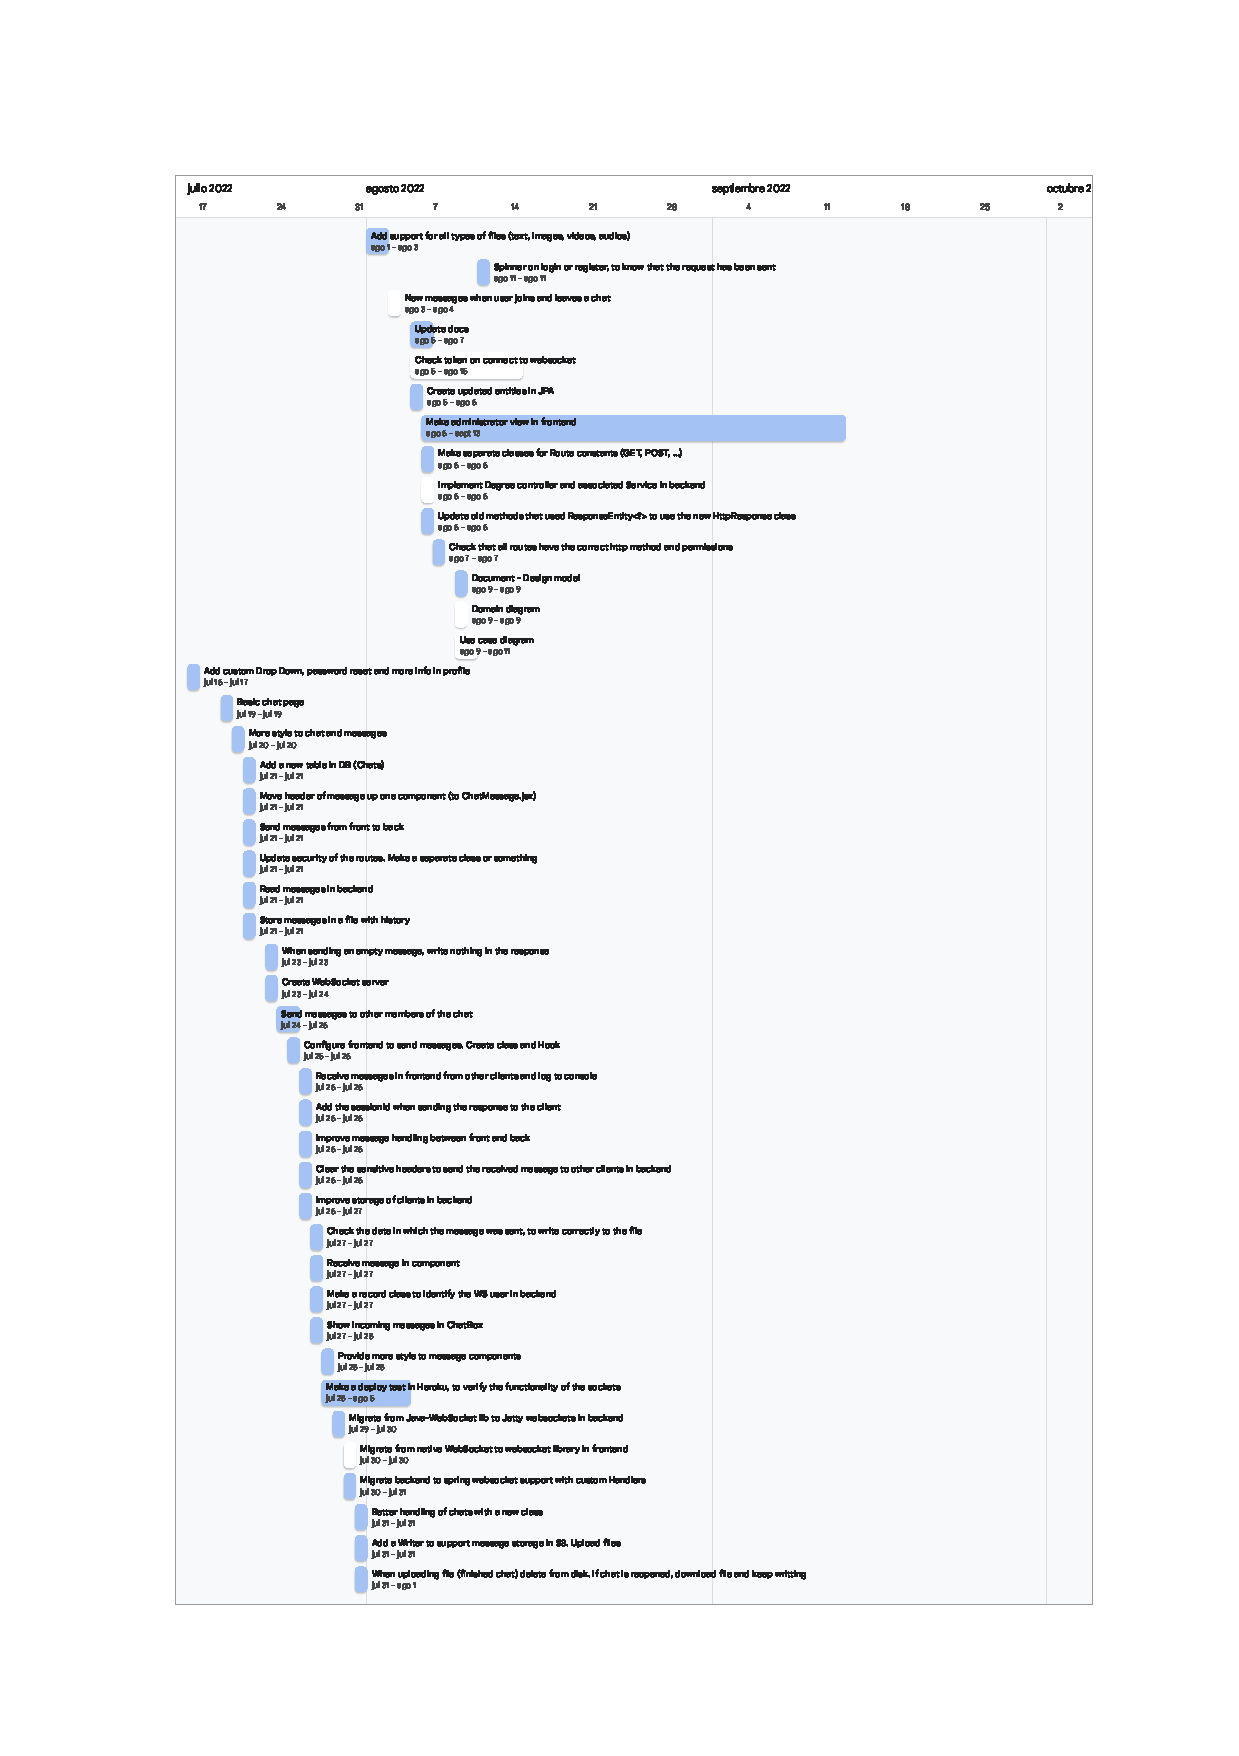
\includepdf[pages=-]{backlog/sprints/Sprint2.pdf}

\subsect{Sprint 3}{sprint3}

Objetivo:

Fecha de inicio: 11/08/2022

Fecha de fin: 11/09/2022

Descripción:

\subsect{Sprint 4}{sprint4}

\underline{Fecha de inicio}: 11/09/2022

\underline{Fecha de fin}: 11/10/2022

\underline{Objetivos}:
\begin{itemize}
	\item Añadir soporte para el envío de archivos.
	\item Utilizar Docker para la aplicación.
\end{itemize}

\underline{Descripción}:
En este sprint se añadirá soporte para el envío de archivos multimedia en los mensajes.\ Se limitará el tamaño de
los archivos a 30 MB, para evitar que se envíen archivos demasiado grandes.\ Además, se utilizará Docker para
la aplicación, de forma que se pueda desplegar fácilmente en cualquier servidor.\ Esto también facilita la integración
entre todos los servicios utilizados en la aplicación, ya que se pueden desplegar todos a la vez con un solo
comando.\ Se ha realizado la migración de la aplicación a un servidor personal, debido a que Heroku ha eliminado
su plan gratuito, como se ha comentado en el sprint anterior.\ Para más información, consultar la
sección~\ref{sec:problems}.

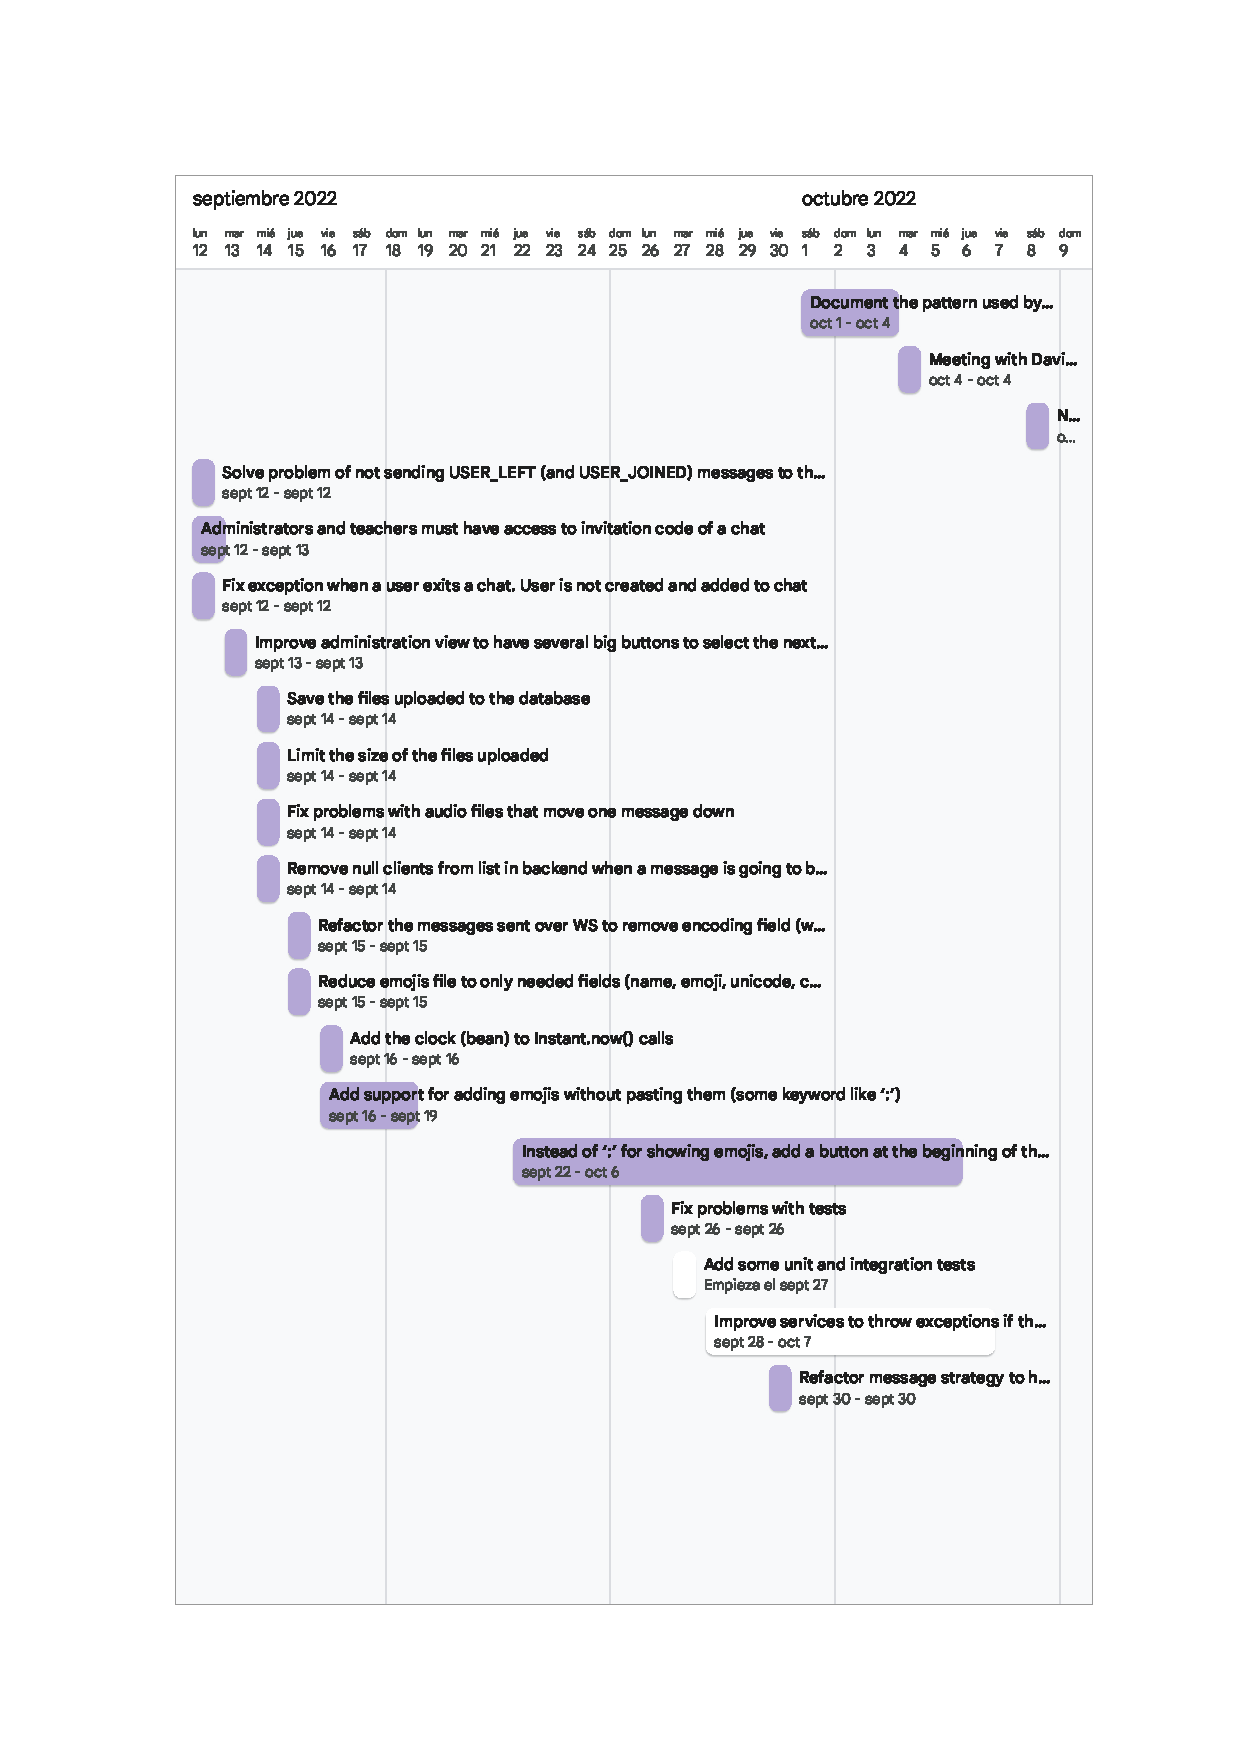
\includepdf[pages=-]{backlog/sprints/Sprint4.pdf}

\subsect{Sprint 5}{sprint5}

\underline{Fecha de inicio}: 11/10/2022

\underline{Fecha de fin}: 11/11/2022

\underline{Objetivos}:
\begin{itemize}
	\item Completar la migración al servidor personal.
	\item Nuevo sistema de menciones.
\end{itemize}

\underline{Descripción}:
En este sprint se añadirá la funcionalidad de menciones, de forma que se pueda mencionar a un usuario en un
mensaje y que este reciba una notificación.\ Además, se completará la migración de la aplicación al servidor
personal.\ Los correos electrónicos que reciben los usuarios se enviarán sin utilizar ningún servicio externo,
ya que hay ocasiones en que ciertos servicios de correo electrónico bloquean los correos que se envían desde
estas plataformas, como SendGrid.\ Debido a esto, se ha creado una cuenta de correo electrónico en Gmail, con el nombre
de la aplicación, y se utilizará para enviar los correos electrónicos.

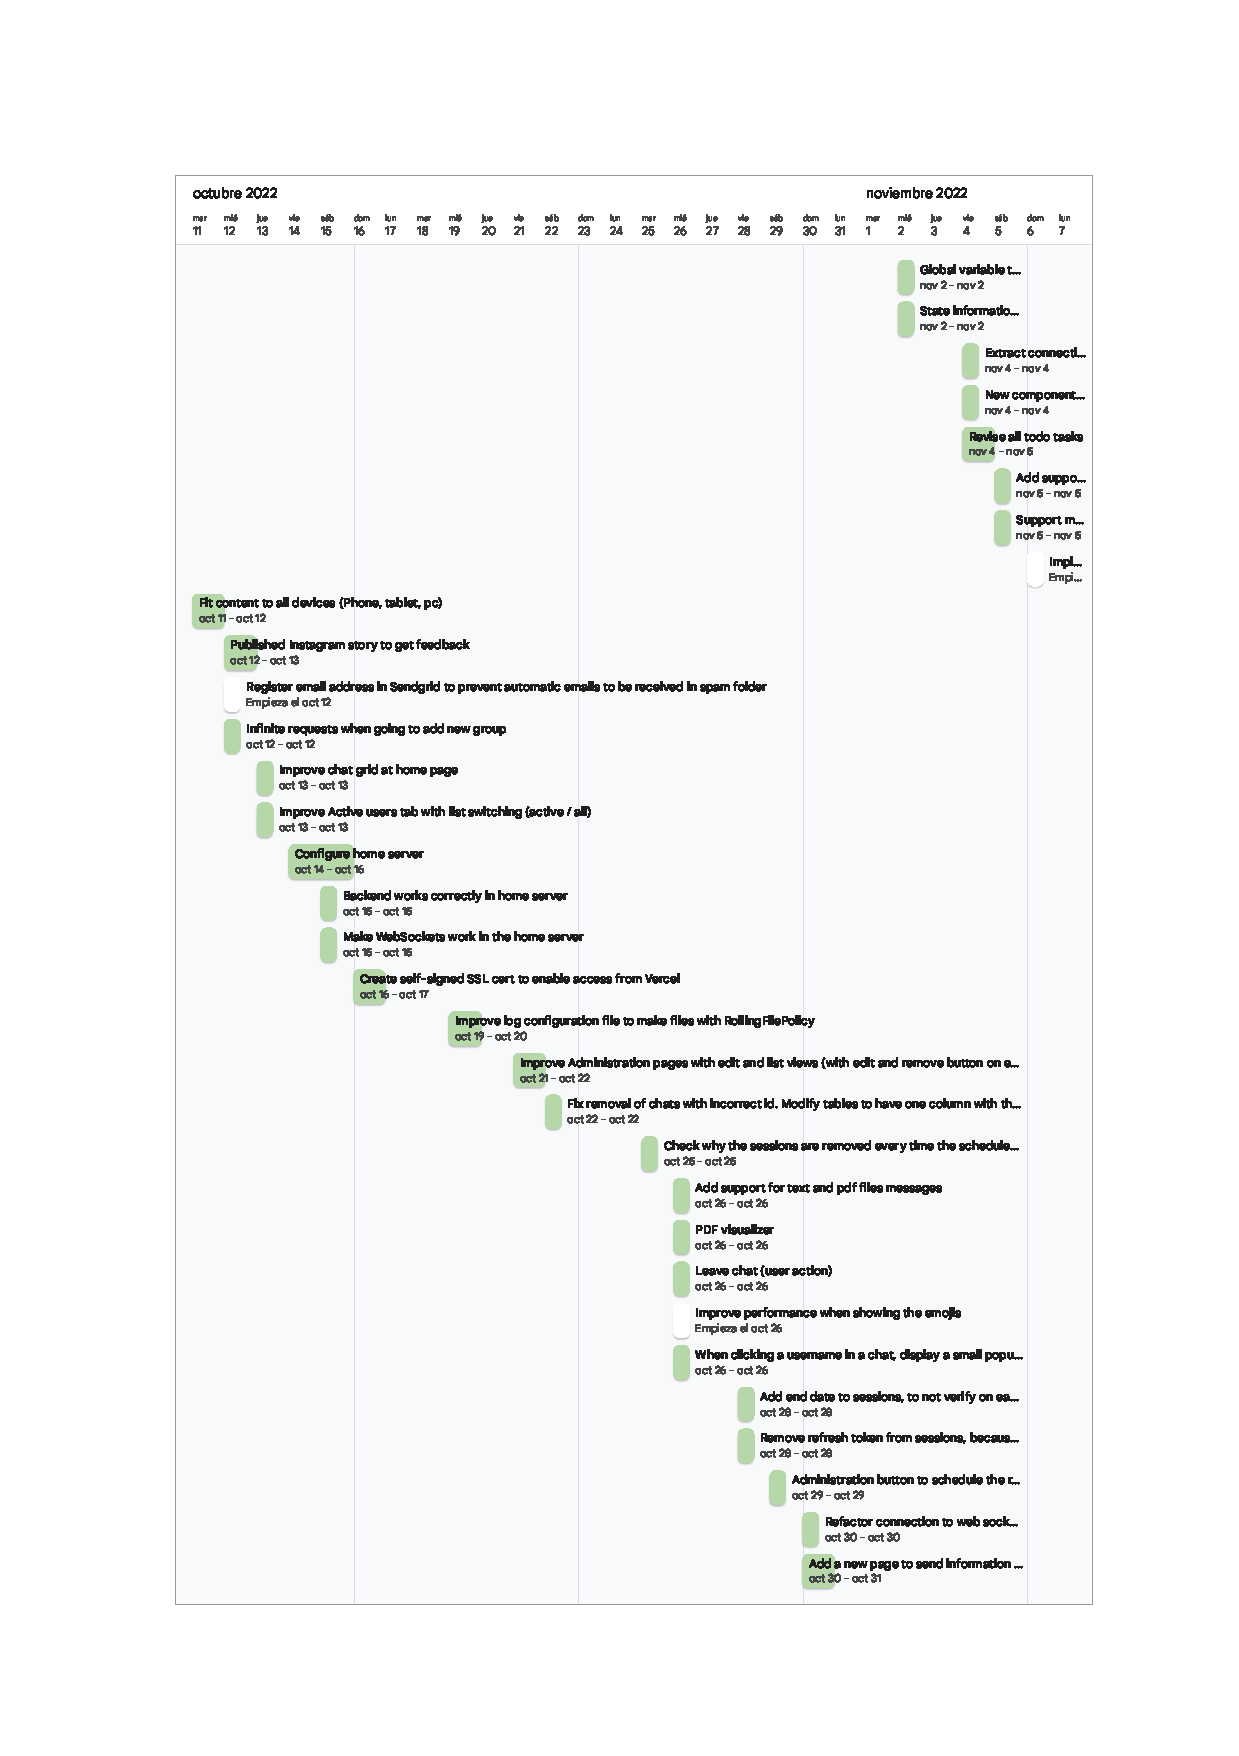
\includepdf[pages=-]{backlog/sprints/Sprint5.pdf}

\subsect{Sprint 6}{sprint6}

\underline{Fecha de inicio}: 11/11/2022

\underline{Fecha de fin}: 11/12/2022

\underline{Objetivo}:
Mejora de la observabilidad del sistema.

\underline{Descripción}:
En este sprint se pretende mejorar la observabilidad del sistema utilizando paneles para su administración.\ Estos
paneles se utilizarán para monitorizar el estado del sistema y para visualizar los datos de los logs obtenidos.
Todo esto conlleva la creación de 3 contenedores Docker adicionales:

\begin{itemize}
	\item Prometheus:
	Sistema de monitorización y alertas.
	\item Grafana:
	Sistema de visualización de datos.
	\item Loki:
	Sistema de logs.
\end{itemize}

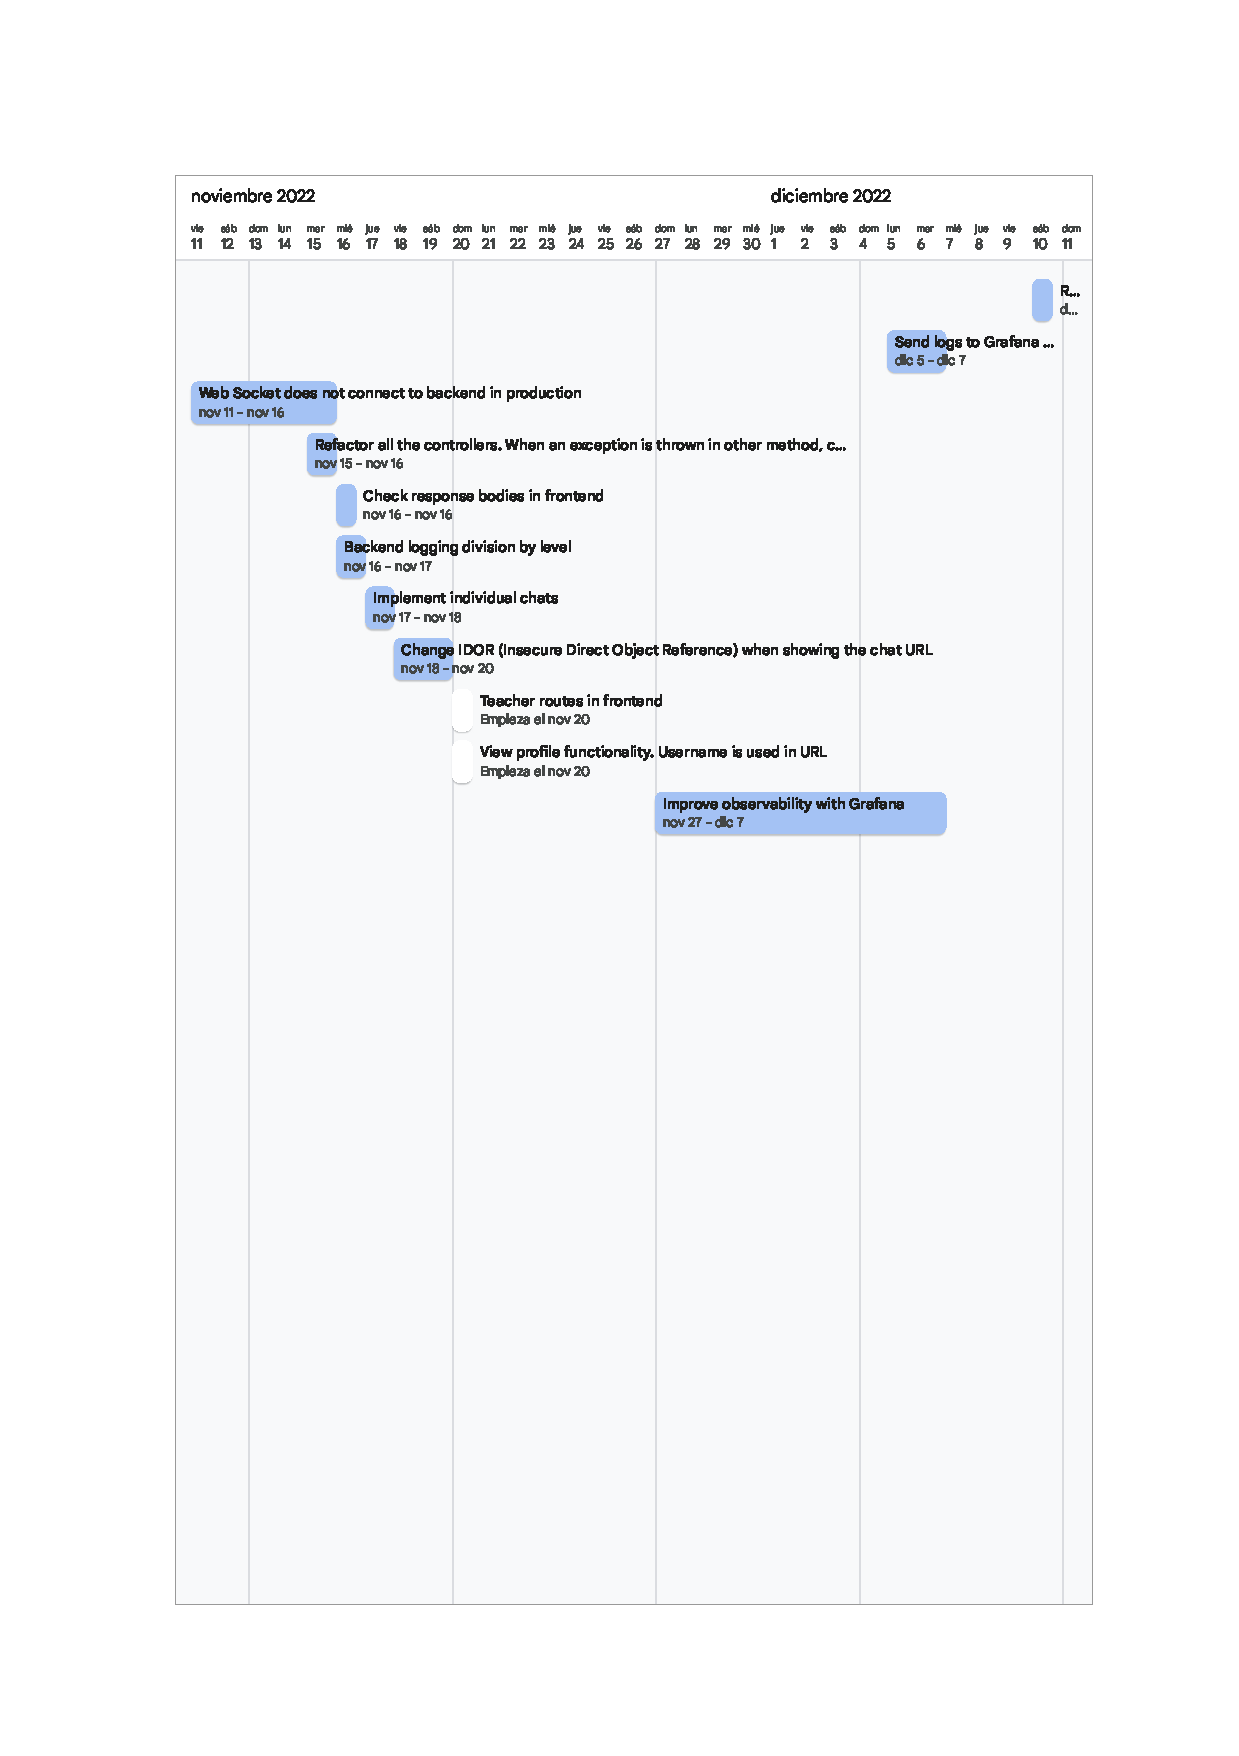
\includepdf[pages=-]{backlog/sprints/Sprint6.pdf}

\subsect{Sprint 7}{sprint7}

\underline{Fecha de inicio}: 11/12/2022

\underline{Fecha de fin}: 11/01/2023

\underline{Objetivo}:
Almacenamiento de estadísticas de mensajes enviados.

\underline{Descripción}:
Para este sprint, se pretenden implementar las estadísticas de mensajes enviados por los usuarios.\ Esto conlleva la
creación de una nueva columna en la tabla \monoFont{users} de la base de datos, que almacenará el número de mensajes
de cada tipo en formato JSON\@.\ Se añadirán nuevos comandos a la aplicación y se modificará su implementación
para soportar múltiples parámetros.

\subsect{Sprint 8}{sprint8}

\underline{Fecha de inicio}: 11/01/2023

\underline{Fecha de fin}: 11/02/2023

\underline{Objetivos}:
\begin{itemize}
	\item \boldFont{Migración de Spring 2.7 a 3.0}
	\item Optimización de la lectura de historiales de mensajes.
	\item Limitación de mensajes enviados por segundo.
\end{itemize}

\underline{Descripción}:
En este sprint se pretende migrar la aplicación a Spring 3.0, ya que añade nuevas mejoras y funcionalidades.
Esta migración conlleva la modificación de la configuración de seguridad de la aplicación y la actualización de las
dependencias a su última versión.

La lectura de mensajes era muy lenta, porque cada vez que un usuario se conectaba,
se descargaba el fichero de mensajes completo.\ Para solucionar esto, se ha implementado un sistema de caché que
almacena los mensajes en memoria.

Para evitar que los usuarios envíen mensajes de forma masiva, se ha implementado un limitador de mensajes por segundo.
Es de implementación propia y se basa en un contador para cada usuario, que se reinicia cada segundo.\ Si el contador
supera el límite, no se permite el envío de mensajes hasta que se reinicie.

\subsect{Sprint 9}{sprint9}

\underline{Fecha de inicio}: 11/02/2023

\underline{Fecha de fin}: 11/03/2023

\underline{Objetivos}:
\begin{itemize}
	\item Mejor implementación de las respuestas HTTP\@.
	\item \boldFont{Uso de un modelo de inteligencia artificial para la detección de imágenes inapropiadas.}
\end{itemize}

\underline{Descripción}:
Para este sprint se realizará un completo rediseño de la implementación de las respuestas HTTP, ya que se debe
facilitar su uso y la creación de nuevas respuestas en cada controlador.

El modelo de inteligencia artificial para la detección de imágenes inapropiadas
que se empleará en la aplicación se ha obtenido del repositorio de GitHub
\href{https://github.com/GantMan/nsfw_model}{\textit{GantMan/nsfw\_model}}~\cite{nsfw-model-repo}.
La implementación de este modelo se realizará en un nuevo servicio utilizando NodeJS y la librería TensorFlowJS\@.

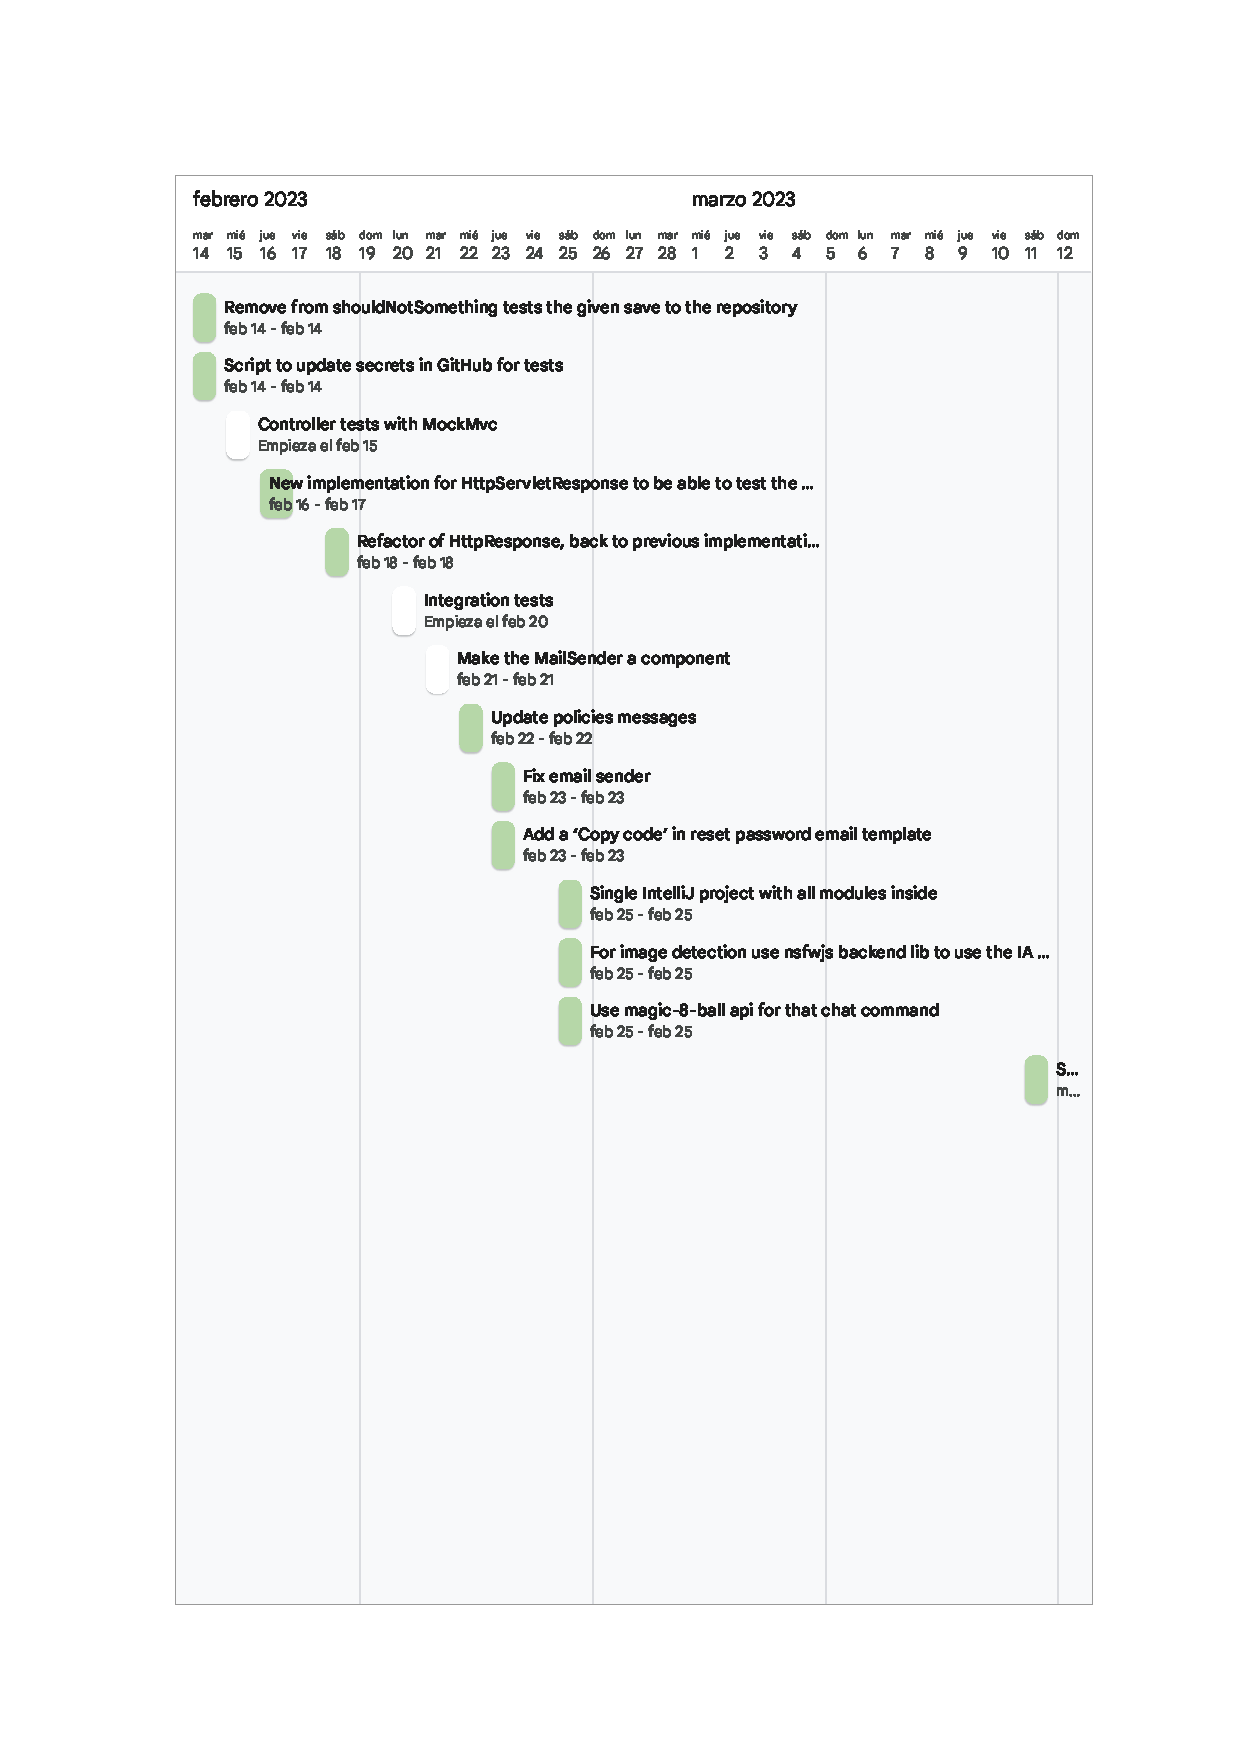
\includepdf[pages=-]{backlog/sprints/Sprint9.pdf}

\subsect{Sprint 10}{sprint10}

Objetivo:

Fecha de inicio: 11/03/2023

Fecha de fin: 11/04/2023

Descripción:

\subsect{Sprint 11}{sprint11}

\underline{Fecha de inicio}: 11/04/2023

\underline{Fecha de fin}: 11/05/2023

\underline{Objetivo}:
Mantenimiento y corrección de errores.

\underline{Descripción}:
A partir de este sprint, el equipo de desarrollo se centrará en la corrección de errores y el mantenimiento del
producto.

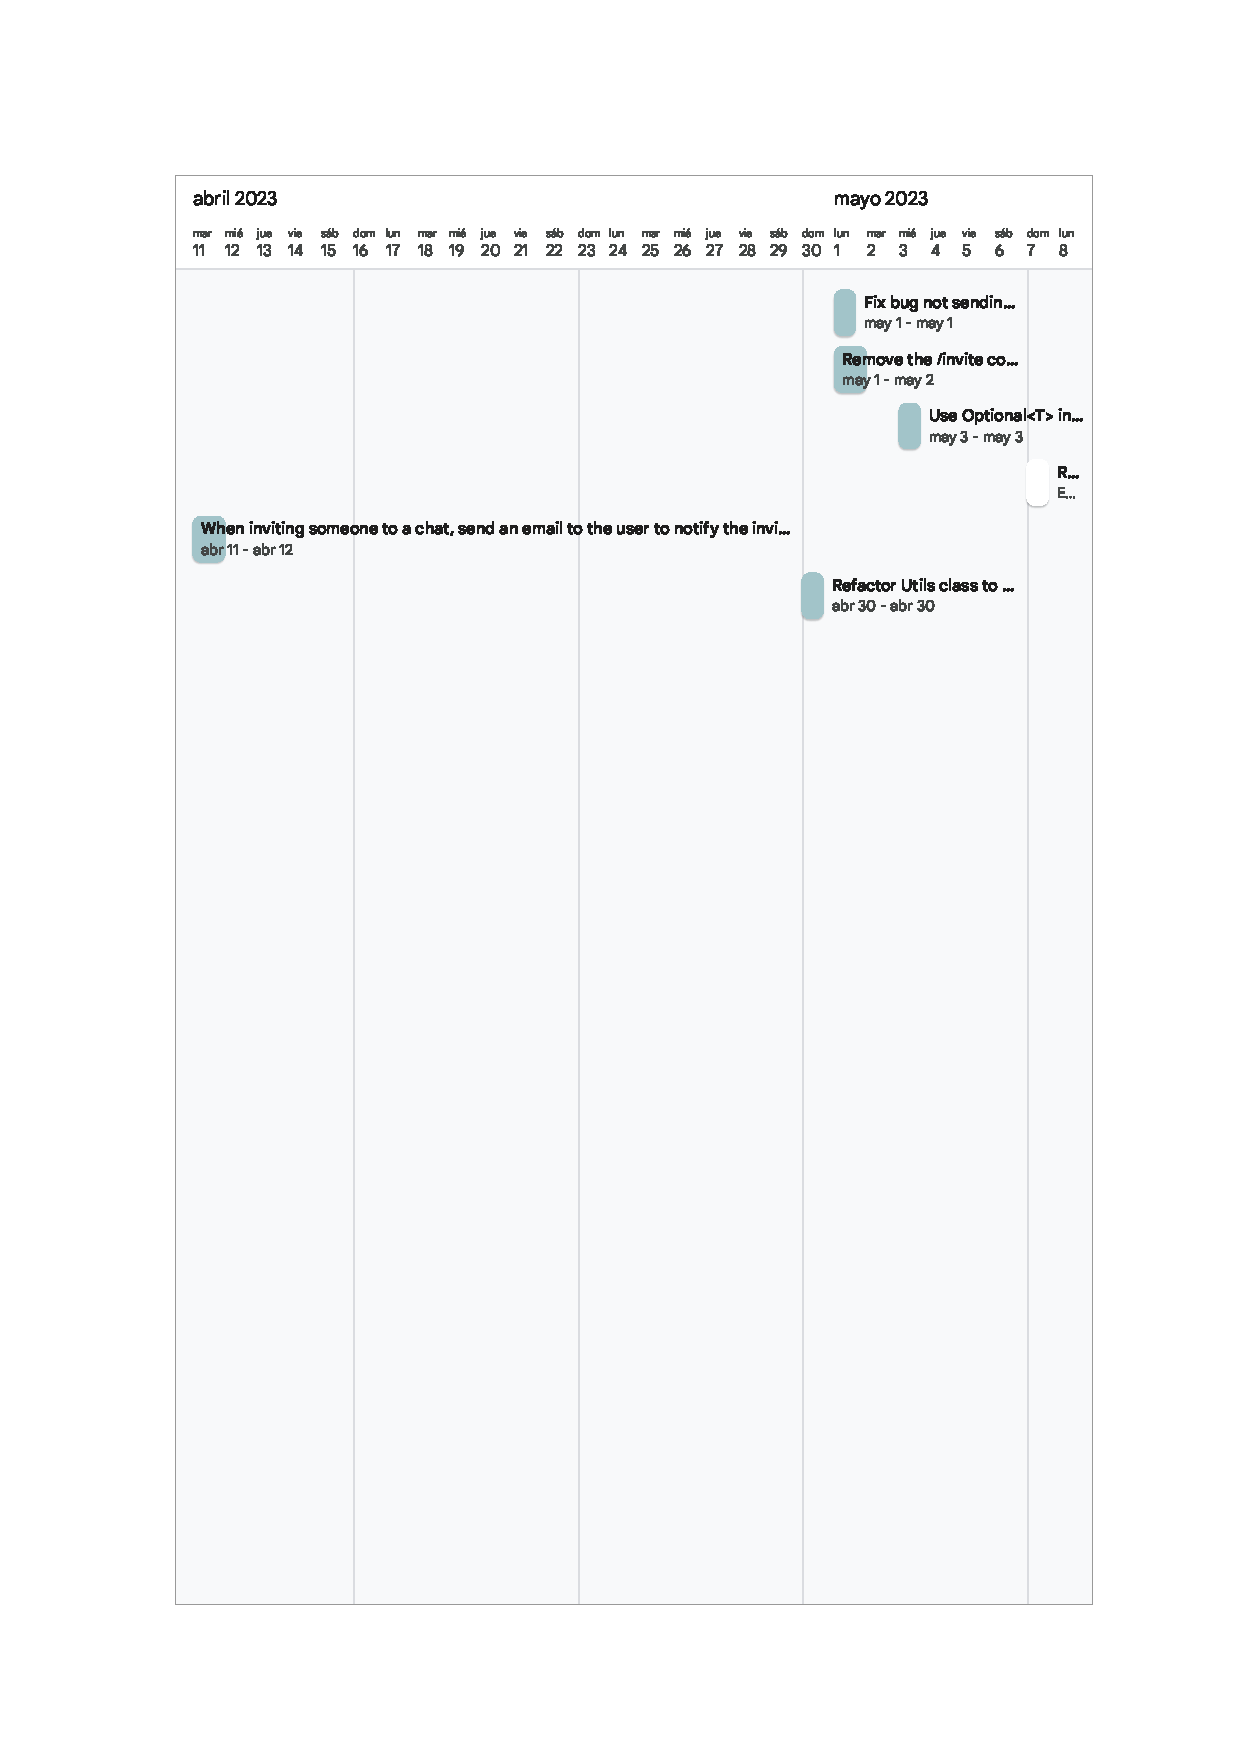
\includepdf[pages=-]{backlog/sprints/Sprint11.pdf}

\subsect{Sprint 12}{sprint12}

Objetivo:

Fecha de inicio: 11/05/2023

Fecha de fin: 11/06/2023

Descripción:


